\documentclass[aps,prresearch,reprint,superscriptaddress,floatfix,amsmath,amssymb]{revtex4-2}

\usepackage{graphicx}
\usepackage{booktabs}
\usepackage{bm}
\usepackage{mathtools}
\usepackage{hyperref}
\usepackage{orcidlink}
\hypersetup{hidelinks}

\newcommand{\dd}{\mathrm{d}}
\newcommand{\ee}{\mathrm{e}}
\newcommand{\ii}{\mathrm{i}}
\newcommand{\Ree}{\operatorname{Re}}
\newcommand{\Imm}{\operatorname{Im}}
\newcommand{\Tr}{\operatorname{Tr}}
\newcommand{\I}{\mathcal{I}}

\begin{document}

\title{Exceptional-point unfolding and critical bare-energy return in a
frequency-swept qubit}

\author{Francisco Ahumada}
\affiliation{Departamento de F\'isica, Universidad T\'ecnica Federico Santa Mar\'ia,
Casilla 110-V, Valpara\'iso, Chile}

\author{Felipe Barra}
\affiliation{Departamento de F\'isica, Facultad de Ciencias F\'isicas y
Matem\'aticas, Universidad de Chile, 837.0415 Santiago, Chile}

\author{Ariel Norambuena\orcidlink{0000-0001-9496-8765}}
\email{ariel.norambuena@usm.cl}
\affiliation{Departamento de F\'isica, Universidad T\'ecnica Federico Santa Mar\'ia,
Casilla 110-V, Valpara\'iso, Chile}

\date{July 15, 2026}

\begin{abstract}
The interplay between time-dependent Hamiltonian control and dissipation is often approximated by an instantaneous Lindblad equation, neglecting reservoir memory and the dynamical phases accumulated during the drive. Here, we analytically solve a two-level system whose transition frequency is modulated in time while it is coupled to an amplitude-damping bosonic reservoir. For a Lorentzian spectral density and a linear detuning ramp, the exact one-excitation dynamics reduces to a Weber equation governing the excited-state population. We show that population revivals coincide interval by interval with a negative time-local decay rate, CP indivisibility, distinguishability backflow, and a positive heat-like contribution to the bare-system energy balance. At fixed resonance, the onset of these effects is governed by a second-order exceptional point separating monotonic relaxation from damped oscillations. A slow sweep turns this sharp threshold into a nonanalytic boundary. For smooth controls with the same local slope, the leading square-root behavior and the next fractional correction are universal and obtained analytically. Finite ramps reveal a crossover to endpoint-controlled revivals and a terminal cusp. Exact energy balances show that a positive heat-like current need not imply either an increase of the total qubit energy or energy lost by the reservoir. An instantaneous Markovian description misses the entire revival domain. These results provide an analytically controlled framework for identifying when coherent control activates reservoir memory and why standard Markovian modeling can predict qualitatively opposite behavior.
\end{abstract}

\maketitle

\section{Introduction}
\label{sec:introduction}

The dynamics of a controlled open quantum system arise from a competition among coherent driving, dissipation, and environmental correlations. A common approach is to describe this evolution using a Lindblad master equation whose coefficients are evaluated at the instantaneous system frequency. This approximation assumes that the environment rapidly loses all information about the previous evolution. When the control varies on a timescale comparable to the reservoir correlation time, however, the environment retains a memory of the frequencies and phases explored by the system. Excitations emitted at different times can then interfere and partially return to the system. The effect of the control cannot be described solely by its instantaneous value, because the environment responds to the history accumulated during the drive.

This memory can manifest itself in several ways. The dynamical map may cease to be divisible into independent memoryless steps, initially distinguishable quantum states may recover part of their distinguishability, and a decaying population may temporarily increase~\cite{Breuer2009,Rivas2010,Bylicka2014}. These phenomena are commonly
associated with non-Markovian dynamics, but they are not generally equivalent. Their energetic interpretation is also nontrivial. Information returning to a system does not necessarily carry energy with it, while a reversal of a heat-like current does not necessarily increase the total system energy~\cite{Strasberg2019,Ptaszynski2022,Picatoste2024,ZambonAdesso2025,
Guarnieri2016,Schmidt2016}. In a driven system, the modulation itself performs work, and at finite coupling a non-negligible amount of energy can be stored in the system-reservoir interaction. A rigorous analysis must therefore distinguish changes of population, work performed by the control, changes of the system energy, and microscopic energy exchange with the reservoir.

Frequency modulation offers a direct way to investigate this interplay. By changing the transition frequency of a two-level system, the control modifies both its instantaneous resonance with the environment and the phase accumulated between emission and reabsorption. This mechanism differs from dynamical decoupling: the interaction is not averaged to zero by a sequence of rapid pulses. Instead, the control continuously reshapes how the system samples the environmental spectrum. Frequency modulation has been used to protect coherence, modify spontaneous emission, and improve reservoir metrology~\cite{Mortezapour2018,Zhang2026,Khazaei2026}, while non-Markovian effects in driven and detuned qubits have been characterized using several complementary measures~\cite{Haikka2011,Li2010,Amati2024}. What remains difficult is to
determine the precise control threshold at which environmental
memory first becomes visible as a population revival.


In this work, we present an exactly solvable mode based on a controlled spin-boson model at zero temperature. We show that a negative time-local decay rate, loss of divisibility, distinguishability backflow, and population revival occur over the same time intervals. At fixed resonance, their onset is governed by a second-order exceptional point separating monotonic relaxation from oscillatory excitation exchange with the effective reservoir mode. A slow frequency sweep unfolds this static threshold into a nonanalytic critical boundary, for which we derive the first two fractional-power contributions analytically and establish their universality for smooth controls with the same local slope. For finite-time protocols, the exact dynamics also reveals when the endpoint of the sweep determines the appearance of the first revival. We finally resolve the thermodynamic meaning of this memory-induced behavior by separating work, heat-like, reservoir, and interaction-energy currents~\cite{TalknerHanggi2020,Campbell2018}. A positive heat-like current can then coexist with a decreasing qubit energy and an energy-gaining reservoir because energy stored in system-reservoir correlations contributes to the balance. An instantaneous Markovian description misses this entire revival region, demonstrating that environmental memory can change both the predicted dynamics and its physical interpretation.

\section{Exact model dynamics in the single-excitation manifold}
\label{sec:model}

\subsection{Hamiltonian symmetry and one-excitation reduction}
Consider a driven two-level system (TLS) coupled to a bosonic reservoir
(\(\hbar=1\)):
\begin{equation}
H(t)=\omega(t)\sigma_+\sigma_-
+\sum_k\omega_k b_k^\dagger b_k
+\sum_k\left(g_k\sigma_+b_k+g_k^*\sigma_-b_k^\dagger\right),
\label{eq:Hamiltonian}
\end{equation}
where \(\omega(t)=\omega_0+f(t)\) is the instantaneous gap,
\(\omega_0\) is the bare gap, \(f(t)\) is the modulation, and \(g_k\) are
the system--environment coupling constants. Here
\(\sigma_+=|e\rangle\langle g|=\sigma_-^\dagger\), while
\(b_k^\dagger\) (\(b_k\)) creates (annihilates) a reservoir boson. Owing to
the global \(U(1)\) symmetry, the excitation-number operator
\(\hat N=\sigma_+\sigma_-+\sum_k b_k^\dagger b_k\) is conserved:
\([H(t),\hat N]=0\) at every time. The total Hilbert space therefore
decomposes into invariant sectors,
\(\mathcal H=\bigoplus_{n=0}^\infty\mathcal H_n\), where
\(\hat N|\psi_n\rangle=n|\psi_n\rangle\). This conservation law remains
exact although \(\omega(t)\) is time dependent, because the drive changes the
excitation energy but neither creates nor
annihilates excitations.

We consider the initial full state \(|\Psi(0)\rangle = |e,0\rangle\), so the dynamics is confined to \(\mathcal H_1\). In the Schr\"odinger picture the most general state in 
that sector is written as $|\Psi(t)\rangle=C_e(t)|e,0\rangle
+\sum_k C_k(t)|g,1_k\rangle$, where \(|1_k\rangle=b_k^\dagger|0\rangle\). The Schr\"odinger equation gives the coupled coefficient equations
\begin{align}
\ii\dot C_e&=\omega(t)C_e+\sum_k g_kC_k,
\nonumber\\
\ii\dot C_k&=\omega_kC_k+g_k^*C_e,
\qquad C_e(0)=1,\quad C_k(0)=0.
\label{eq:Schrodingercoefficients}
\end{align}
Let \(\Phi(t)=\int_0^t\omega(v)\dd v\) be the dynamical phase, and remove
the free phases through
\begin{equation}
C_e(t)=c(t)\ee^{-\ii\Phi(t)},
\qquad C_k(t)=\beta_k(t)\ee^{-\ii\omega_kt}.
\label{eq:interactionamplitudes}
\end{equation}
The coefficient equations then become
\begin{align}
\dot c(t)&=-\ii\sum_k g_k\beta_k(t)
\ee^{-\ii[\omega_kt-\Phi(t)]},
\nonumber\\
\dot\beta_k(t)&=-\ii g_k^*c(t)
\ee^{\ii[\omega_kt-\Phi(t)]}.
\label{eq:interactioncoefficients}
\end{align}
Integrating the second line with \(\beta_k(0)=0\) and substituting it back
gives the exact Volterra equation
\begin{align}
\dot c(t)&=-\int_0^t\mathcal K(t,u)c(u)\dd u,
\label{eq:discreteVolterra}\\
\mathcal K(t,u)&=\sum_k|g_k|^2
\exp\!\left[-\ii\omega_k(t-u)
+\ii\int_u^t\omega(v)\dd v\right].
\label{eq:discretekernel}
\end{align}
No Born, Markov, secular, or continuum approximation has entered this
reduction, so Eqs.~\eqref{eq:discreteVolterra} and
\eqref{eq:discretekernel} give the exact dynamics in the single-excitation
manifold. The time-dependent gap makes the kernel nonstationary: in general,
\(\mathcal K(t,u)\neq\mathcal K(t-u)\). The phase transformation does not
change the probability \(|c(t)|^2\). Tracing out the bosonic degrees of
freedom gives the system density matrix
\begin{equation}
\rho_S(t)=P(t)\lvert e\rangle\langle e\rvert
+[1-P(t)]\lvert g\rangle\langle g\rvert,
\qquad P(t)=|c(t)|^2.
\label{eq:rhoS}
\end{equation}

\subsection{Lorentzian reservoir and pseudomode embedding}

We now take the continuum limit by specifying the coupling distribution
through the Lorentzian spectral density
\begin{equation}
J_L(\nu) \equiv \sum_k|g_k|^2\delta_{\rm D}(\nu-\omega_k)
=\frac{\gamma_0\lambda^2}
{2\pi[(\nu-\omega_b)^2+\lambda^2]}.
\label{eq:Lorentziandensity}
\end{equation}
Here, \(\omega_b\) is the center of the reservoir line, \(\lambda^{-1}\) is
its correlation time, and \(\gamma_0\) fixes the overall coupling scale; no
weak-coupling or Born approximation is imposed below. In general
\(\omega_b\) is not the TLS gap; their difference defines the controlled
detuning below. The effective full-line Lorentzian extension, its
positive-frequency limit, the reconstruction of the discrete coefficients
\(g_k\), and the exact
reservoir amplitudes are detailed in the Supplemental
Material~\cite{SupplementalMaterial}.
Factoring
the phase at \(\omega_b\) in Eq.~\eqref{eq:discretekernel} defines
\begin{equation}
\delta(t) \equiv \omega_b-\omega(t)
\label{eq:detuningdefinition}
\end{equation}
and the stationary bath correlation function
\begin{align}
f_L(s)&=\int_{-\infty}^{\infty}J_L(\nu)
\ee^{-\ii(\nu-\omega_b)s}\dd\nu =\frac{\gamma_0\lambda}{2}\ee^{-\lambda s},
\qquad s\geq0.
\label{eq:Lorentziankernel}
\end{align}
The integral over the full real line defines an effective Lorentzian reservoir in
rotating detuning coordinates; it is not literally identical to a bosonic
Hamiltonian bounded below by \(\nu=0\). The fraction of the Lorentzian weight
retained at positive laboratory frequencies is
\begin{equation}
\eta_+=\frac{\int_0^\infty J_L(\nu)\dd\nu}
{\int_{-\infty}^\infty J_L(\nu)\dd\nu}
=\frac12+\frac{1}{\pi}\arctan\!\left(\frac{\omega_b}{\lambda}\right).
\label{eq:positiveweight}
\end{equation}
Accordingly, the exponential kernel and the one-pseudomode representation are
exact for this effective full-line Lorentzian reservoir, while they approximate
a positive-frequency reservoir in the controlled carrier limit
\(\omega_b/\lambda\gg1\). We keep this carrier scale independent of the
detuning range below.
Thus, the exact TLS equation can be written as
\begin{equation}
\dot c(t)=-\int_0^t f_L(t-u)
\exp\!\left[-\ii\int_u^t\delta(v)\dd v\right]c(u)\dd u.
\label{eq:atomicVolterra}
\end{equation}
This step displays precisely where the spectral density enters: the
Hamiltonian symmetry first reduces the dynamics to one amplitude, and the
choice of \(J_L\) then fixes its memory kernel. The protocol starts exactly
at the Lorentzian center, \(\omega(0)=\omega_b\), and lowers the gap linearly
over a range \(\Delta_f\), while maintaining a positive final gap
\(\omega_f=\omega_b-\Delta_f>0\).
In terms of \(\omega(t)=\omega_0+f(t)\), this initial resonance means
\(f(0)=\omega_b-\omega_0\); it does not require \(\omega_0=\omega_b\).
\begin{align}
\omega(t)&=\omega_b-\alpha t,
\qquad \delta(t)=\alpha t,
\label{eq:linearprotocol}
\end{align}
where
\begin{equation}
\Delta_f=\omega_b-\omega_f,\qquad
0\leq t\leq t_f=\frac{\Delta_f}{\alpha},\qquad \omega_f>0.
\label{eq:finiteprotocol}
\end{equation}
The static reference problem \(a=0\) used below is therefore a qubit held
exactly on resonance, \(\omega(t)=\omega_b\), rather than a separately chosen
static gap. We introduce the independent dimensionless carrier and sweep
range
\begin{equation}
\begin{aligned}
\tau&=\gamma_0t,&
\ell&=\frac{\lambda}{\gamma_0},&
a&=\frac{\alpha}{\gamma_0^2},\\
\Omega_b&=\frac{\omega_b}{\gamma_0},&
\Omega_\Delta&=\frac{\Delta_f}{\gamma_0},&
\tau_f&=\frac{\Omega_\Delta}{a}.
\end{aligned}
\label{eq:dimensionless}
\end{equation}
The physical regime used for energetic and experimental statements obeys
\(\Omega_b>\Omega_\Delta\) and \(\Omega_b/\ell\gg1\); neither condition
changes the reduced equation because it depends only on the detuning
\(\delta(\tau)=a\tau\).
The Hamiltonian also assumes that tuning the gap does not rotate the TLS
eigenbasis or change the magnitudes and phases of \(g_k\). This is exact
within Eq.~\eqref{eq:Hamiltonian}; experimentally it requires either a
longitudinal frequency control or a sufficiently small fractional sweep that
any coupling variation can be calibrated perturbatively.
Because Eq.~\eqref{eq:Lorentziankernel} is a single exponential, its entire
memory integral can be stored in one auxiliary amplitude, giving the exact
pseudomode embedding~\cite{Garraway1997,Pleasance2020}. Setting
\(g=\sqrt{\ell/2}\) and defining
\begin{align}
b(\tau)&=-\ii g\int_0^\tau\ee^{-\ell(\tau-u)}
\exp\!\left[-\frac{\ii a}{2}(\tau^2-u^2)\right]c(u)\dd u.
\label{eq:pseudomodedefinition}
\end{align}
Equation~\eqref{eq:atomicVolterra} gives the first equation below, while
differentiating Eq.~\eqref{eq:pseudomodedefinition} gives the second. Thus
the Lorentzian reservoir correlation function is exactly equivalent to damped
pseudomode dynamics:
\begin{align}
c'&=-\ii g b,\nonumber\\
b'&=-(\ell+\ii a\tau)b-\ii g c,
\label{eq:pseudomode}
\end{align}
where a prime denotes \(\dd/\dd\tau\). Defining the amplitude vector
\begin{equation}
\bm v(\tau)=
\begin{pmatrix}
c(\tau)\\
b(\tau)
\end{pmatrix},
\end{equation}
the pseudomode equations take the Schr\"odinger-like form
\begin{equation}
\ii\frac{\dd}{\dd\tau}\bm v(\tau)
=H_{\rm eff}(\tau)\bm v(\tau),
\qquad
H_{\rm eff}(\tau)=
\begin{pmatrix}
0 & g\\
g & a\tau-\ii\ell
\end{pmatrix}.
\label{eq:Heff}
\end{equation}
The exact non-Markovian qubit dynamics is therefore embedded into a
two-dimensional evolution generated by an effective non-Hermitian Hamiltonian.
Its non-Hermiticity is not introduced phenomenologically: the term
\(-\ii\ell\) represents irreversible leakage from the pseudomode into the
residual Markovian environment. Indeed,
\begin{equation}
\frac{\dd}{\dd\tau}\left(\bm v^\dagger\bm v\right)
=\ii\bm v^\dagger
\left(H_{\rm eff}^\dagger-H_{\rm eff}\right)\bm v
=-2\ell|b|^2\leq0.
\label{eq:pseudomodenorm}
\end{equation}
Thus, the loss of norm in the qubit--pseudomode sector is precisely the
probability irreversibly transferred to the residual environment.
Here, \(H_{\rm eff}\) is the exact amplitude generator in the
one-excitation sector, equivalently the no-jump generator of the Markovian
embedding. Eliminating \(b\) gives the exact scalar equation
\begin{equation}
c''+(\ell+\ii a\tau)c'+\frac{\ell}{2}c=0,
\qquad c(0)=1,\quad c'(0)=0.
\label{eq:exactODE}
\end{equation}

\subsection{Weber solution and exact logarithmic derivative}

For \(a>0\), Eq.~\eqref{eq:exactODE} can be reduced explicitly to the
Weber equation. Writing \(p(\tau)=\ell+\ii a\tau\), we apply the standard
integrating-factor transformation
\begin{align}
c(\tau)
&=\exp\!\left[-\frac12\int_0^\tau p(u)\dd u\right]y(\tau)\nonumber\\
&=\exp\!\left(-\frac{\ell\tau}{2}
-\frac{\ii a\tau^2}{4}\right)y(\tau).
\label{eq:gaugetransform}
\end{align}
For a general equation \(c''+pc'+rc=0\), this transformation yields
\(y''+[r-p'/2-p^2/4]y=0\). Equation~\eqref{eq:exactODE} therefore becomes
\begin{equation}
y''+
\left[
\frac{(a\tau-\ii\ell)^2}{4}
+\frac{\ell}{2}
-\frac{\ii a}{2}
\right]y=0.
\label{eq:preWeber}
\end{equation}
Introducing
\begin{equation}
z=\ee^{-\ii\pi/4}\sqrt a
\left(\tau-\frac{\ii\ell}{a}\right),
\qquad
\nu=\frac{\ii\ell}{2a},
\label{eq:Weberparameters}
\end{equation}
and using \(\dd^2/\dd\tau^2=-\ii a\,\dd^2/\dd z^2\), we obtain the
standard Weber equation
\begin{equation}
\frac{\dd^2y}{\dd z^2}
+\left(\nu+\frac12-\frac{z^2}{4}\right)y=0.
\label{eq:standardWeber}
\end{equation}
Its general solution gives
\begin{equation}
c(\tau)=\ee^{-\ell\tau/2-\ii a\tau^2/4}
\left[A D_\nu(z)+B D_\nu(-z)\right],
\label{eq:Webersolution}
\end{equation}
where \(D_\nu\) is a parabolic-cylinder function~\cite{NIST2010} and \(A,B\)
are fixed by the initial conditions. Explicit formulas are given in
Appendix~\ref{app:weber}. Thus, a sequence of exact transformations maps the
driven dissipative one-excitation problem with Lorentzian memory onto a Weber
equation with complex parameters, encoding detuning and irreversible
dissipation. We now define the logarithmic derivative
\begin{equation}
q(\tau)=\frac{c'(\tau)}{c(\tau)},
\label{eq:qdefinition}
\end{equation}
which obeys the exact Riccati equation
\begin{equation}
q'+q^2+(\ell+\ii a\tau)q+\frac{\ell}{2}=0,
\qquad q(0)=0.
\label{eq:Riccati}
\end{equation}
On every interval where \(c\neq0\), the dimensionless decay rate and Lamb
shift are defined as
\begin{equation}
\begin{aligned}
\bar\gamma(\tau)\equiv \frac{\gamma(\tau)}{\gamma_0}
&=-2\Ree\{q(\tau)\},\\
\bar s(\tau)\equiv \frac{s(\tau)}{\gamma_0}
&=-\Imm\{q(\tau)\}.
\end{aligned}
\label{eq:rateandshift}
\end{equation}
Although \(q\) is singular at an isolated zero of \(c(\tau)\), the microscopic
equations and the channel remain regular. On every interval where \(c\neq0\),
the reduced map is invertible and admits the exact time-local amplitude-damping
master equation
\begin{align}
\frac{\dd\rho_{S,I}}{\dd\tau}
={}&-\ii\left[
\bar s(\tau)\sigma_+\sigma_-,\rho_{S,I}(\tau)
\right]\nonumber\\
&+\bar\gamma(\tau)
\left[
\sigma_-\rho_{S,I}(\tau)\sigma_+
-\frac12\left\{\sigma_+\sigma_-,\rho_{S,I}(\tau)\right\}
\right],
\label{eq:exactTimeLocalME}
\end{align}
where \(\rho_{S,I}\) denotes the reduced state in the interaction picture
defined by removing the bare dynamical phase generated by
\(\omega(t)\sigma_+\sigma_-\). The quantities in
Eq.~\eqref{eq:rateandshift} are therefore the exact time-local decay rate and
Lamb-shift correction, respectively. In particular,
\begin{align}
\rho_{ee}'&=-\bar\gamma\rho_{ee},\nonumber\\
\rho_{eg}'&=-\left(\frac{\bar\gamma}{2}+\ii\bar s\right)\rho_{eg}
=q\rho_{eg},
\label{eq:timeLocalComponents}
\end{align}
because \(q=-\bar\gamma/2-\ii\bar s\). For the initially excited reference
state, \(P'=-\bar\gamma P\). When \(\bar\gamma<0\), this exact time-local
representation remains valid but its generator is not of GKSL form.

\section{Operational and energetic meaning of a revival}
\label{sec:operational}

\subsection{Full amplitude-damping map}

The reduced map for an arbitrary qubit input is the standard
amplitude-damping channel~\cite{BreuerPetruccione2002},
\begin{equation}
\Lambda_\tau(\rho)=
\begin{pmatrix}
P\rho_{ee}&c\rho_{eg}\\
c^*\rho_{ge}&\rho_{gg}+(1-P)\rho_{ee}
\end{pmatrix}.
\label{eq:ADmap}
\end{equation}
For \(c(\tau_1)\neq0\), the intermediate map has amplitude
\(c(\tau_2)/c(\tau_1)\) and is completely positive if and only if
\(P(\tau_2)\leq P(\tau_1)\). The same sign controls every nontrivial trace
distance. Explicitly, let \(\rho_1(0)\) and \(\rho_2(0)\) be any two initial
qubit states and define their evolved trace distance by
\begin{equation}
D_{12}(\tau) \equiv \frac12
\left\|\Lambda_\tau[\rho_1(0)-\rho_2(0)]\right\|_1,
\label{eq:tracedistancedefinition}
\end{equation}
where \(\|X\|_1=\Tr\sqrt{X^\dagger X}\). A positive derivative
\(D_{12}'=\dd D_{12}/\dd\tau\) is the Breuer--Laine--Piilo (BLP) signature of information returning
to the system. Write the two initial states in Bloch form,
\begin{equation}
\rho_j(0)=\frac12\left(\mathbb{I}_2+\bm r_j\cdot\bm\sigma\right),
\qquad
\bm r_j\in\mathbb R^3,\quad |\bm r_j|\leq1,
\end{equation}
where \(\bm\sigma=(\sigma_x,\sigma_y,\sigma_z)\) is the Pauli vector in the
basis \(\{|e\rangle,|g\rangle\}\), with
\(\sigma_z=|e\rangle\langle e|-|g\rangle\langle g|\). If
\(\Delta\bm r=\bm r_1-\bm r_2\) is the difference of the two initial Bloch
vectors, define
\begin{equation}
A=(\Delta r_x)^2+(\Delta r_y)^2,
\qquad B=(\Delta r_z)^2.
\end{equation}
Then
\begin{align}
D_{12}(\tau)&=\frac12\sqrt{PA+P^2B},
\label{eq:tracedistance}\\
D_{12}'(\tau)&=
\frac{P'(A+2PB)}{4\sqrt{PA+P^2B}}.
\label{eq:tracedistancerate}
\end{align}
Thus, no optimization over state pairs changes the sign boundary. This yields
the following proposition.

\paragraph{Proposition 1 (equivalence of regular non-Markovianity witnesses).}
Let \(\mathcal I\subset\mathbb R_+\) be an open interval such that
\(c(\tau)\neq0\) for every \(\tau\in\mathcal I\). Then the reduced
amplitude-damping map is invertible and differentiable on \(\mathcal I\), and
for every \(\tau\in\mathcal I\),
\begin{equation}
\begin{aligned}
\Ree\{q(\tau)\}>0
&\Longleftrightarrow \bar\gamma(\tau)<0,\\
&\Longleftrightarrow P'(\tau)>0,\\
&\Longleftrightarrow
\mathcal L_\tau\ \text{is not of GKSL form}.
\end{aligned}
\label{eq:operationalequivalence}
\end{equation}
where \(\mathcal L_\tau\) is the exact time-local generator in
Eq.~\eqref{eq:exactTimeLocalME}. Moreover, for every pair of distinct initial
states \(\rho_1(0)\neq\rho_2(0)\),
\begin{equation}
\operatorname{sgn}D_{12}'(\tau)=\operatorname{sgn}P'(\tau),
\qquad \tau\in\mathcal I.
\label{eq:traceDistanceSignEquivalence}
\end{equation}
Consequently, the Rivas--Huelga--Plenio criterion of CP indivisibility and the
Breuer--Laine--Piilo criterion of distinguishability backflow identify exactly
the same set of regular time intervals for this amplitude-damping dynamics.

\textit{Proof.}
Since \(P=|c|^2\) and \(q=c'/c\),
\begin{equation}
P'=c'c^*+c(c')^*=2P\Ree\{q\}=-\bar\gamma P.
\label{eq:populationRateIdentity}
\end{equation}
Because \(c\neq0\) on \(\mathcal I\), one has \(P>0\), which proves the
first three equivalences in Eq.~\eqref{eq:operationalequivalence}. The exact
time-local amplitude-damping generator has a single canonical dissipative
rate, \(\bar\gamma\). It is therefore of GKSL form at time \(\tau\) if and
only if \(\bar\gamma(\tau)\geq0\), proving the last equivalence. For two
distinct initial states, \(A+B>0\). Since \(P>0\), the denominator in
Eq.~\eqref{eq:tracedistancerate} is strictly positive and \(A+2PB>0\).
Therefore, \(D_{12}'\) has the same sign as \(P'\) for every distinct initial
pair, proving Eq.~\eqref{eq:traceDistanceSignEquivalence}.
\hfill\(\square\)

The restriction \(c\neq0\) is essential. At an isolated zero
\(c(\tau_0)=0\), the map is noninvertible and sends every input to the ground
state; the time-local rate and the ratio defining the intermediate amplitude
are then undefined. Equation~\eqref{eq:tracedistancerate} also has a kinematic
zero-over-zero form because all instantaneous trace distances vanish. No sign
is assigned at \(\tau_0\) itself. If \(P\) becomes positive immediately
afterwards, however, no CPTP propagator can recover distinct outputs from that
fixed state, and CP indivisibility is detected on the adjacent regular
interval. Thus, isolated zeros are handled through the continuous population
and microscopic channel rather than by extending \(q\) through its pole.

\subsection{Bare-system and microscopic energy balances}

We now determine the energetic content of the equivalent non-Markovianity
witnesses established in Proposition~1. Let
\begin{equation}
H_S(t)=\omega(t)n_S,
\qquad n_S=\sigma_+\sigma_-,
\end{equation}
and denote the instantaneous excited-state population by
\(p_e(t)=\Tr[n_S\rho_S(t)]\). For the vacuum amplitude-damping channel,
\begin{equation}
p_e(t)=p_e(0)P(t),
\label{eq:generalExcitedPopulation}
\end{equation}
so \(p_e=P\) for the initially excited reference state. The bare-system energy
is
\begin{equation}
U_S(t)=\Tr[H_S(t)\rho_S(t)]=\omega(t)p_e(t).
\label{eq:bareSystemEnergy}
\end{equation}
Its time derivative admits the exact kinematic decomposition
\begin{align}
\dot U_S
&=\Tr[\dot H_S\rho_S]+\Tr[H_S\dot\rho_S]
\equiv\dot W_S+\dot Q_S,
\label{eq:systemenergybalance}
\end{align}
where
\begin{equation}
\dot W_S=\dot\omega\,p_e,
\qquad
\dot Q_S=\omega\dot p_e=-\omega\gamma p_e.
\label{eq:workheat}
\end{equation}
Here, \(\dot W_S\) is the power supplied by the frequency modulation, whereas
\(\dot Q_S\) is the heat-like contribution associated with population
changes. Equation~\eqref{eq:systemenergybalance} is an exact identity for the
bare system. At finite coupling, however, \(\dot Q_S\) must not be identified
a priori with energy lost by the reservoir.

For the initially excited state and the descending linear sweep,
\(\omega/\gamma_0=\Omega_b-a\tau>0\), one obtains
\begin{align}
\frac{\dot U_S}{\gamma_0^2}
&=P\left[-a-(\Omega_b-a\tau)\bar\gamma\right],
\nonumber\\
\dot U_S>0
&\Longleftrightarrow
-\bar\gamma>\frac{a}{\Omega_b-a\tau}.
\label{eq:systemenergyrate}
\end{align}
Thus, a population revival does not by itself guarantee an increase of the
total bare-system energy: the positive population contribution must also
overcome the negative work rate associated with the descending sweep.

\paragraph{Proposition 2 (energetic content of a revival).}
On a regular interval where \(c\neq0\), assume \(\omega(t)>0\) and
\(p_e(0)>0\). Then
\begin{equation}
\Ree\{q\}>0
\Longleftrightarrow \bar\gamma<0
\Longleftrightarrow \dot p_e>0
\Longleftrightarrow \dot Q_S>0.
\label{eq:energybackflow}
\end{equation}
No corresponding implication holds in general for either \(\dot U_S>0\) or
\(-\dot E_B>0\).

\textit{Proof.}
Equation~\eqref{eq:generalExcitedPopulation} and Proposition~1 give
\(\dot p_e=-\gamma p_e\). Since \(p_e>0\) on the regular interval and
\(\omega>0\), \(\dot Q_S=-\omega\gamma p_e\) has the opposite sign to
\(\gamma\), proving Eq.~\eqref{eq:energybackflow}. On the other hand,
\(\dot U_S=\dot W_S+\dot Q_S\) contains the independent control-work
contribution. Likewise, the microscopic balance below contains the
interaction-energy current in addition to the reservoir current. Therefore,
neither \(\dot U_S>0\) nor \(-\dot E_B>0\) follows from \(\dot Q_S>0\).
\hfill\(\square\)

To resolve the microscopic origin of \(\dot Q_S\), partition the total
Hamiltonian as \(H(t)=H_S(t)+H_B+V\) and define
\(E_B(t)=\langle H_B\rangle_t\) and \(E_I(t)=\langle V\rangle_t\). Because the
external time dependence enters only through \(H_S(t)\), unitary evolution of
the complete system gives the exact first law
\begin{equation}
\frac{\dd}{\dd t}\left[U_S(t)+E_B(t)+E_I(t)\right]
=\left\langle\frac{\partial H(t)}{\partial t}\right\rangle
=\dot W_S(t).
\label{eq:microscopicFirstLaw}
\end{equation}
Combining this identity with Eq.~\eqref{eq:systemenergybalance} yields
\begin{equation}
\dot Q_S=-\dot E_B-\dot E_I.
\label{eq:strongbalance}
\end{equation}
Therefore, the heat-like bare-system current is balanced by the combined
change of reservoir and interaction energies, rather than by the reservoir
energy alone. For the pure reference state
\(|\Psi(0)\rangle=|e,0\rangle\), the interaction energy follows directly from
the exact amplitude equations:
\begin{align}
E_I(t)
&=-2\Imm\!\left[c^*(t)\dot c(t)\right]\nonumber\\
&=-2P(t)\Imm\!\left\{\frac{\dot c(t)}{c(t)}\right\}
=2P(t)s(t).
\label{eq:interactionenergy}
\end{align}
The first expression remains regular even at an isolated zero of \(c\).
Equation~\eqref{eq:interactionenergy} establishes an exact relation between
the Lamb-shift correction in the time-local generator and the energy stored in
the system--reservoir interaction. Taking the vacuum energy as zero, the
initial total energy is \(\omega(0)\). Integrating
Eq.~\eqref{eq:microscopicFirstLaw} then gives
\begin{equation}
E_B(t)=\omega(0)+\int_0^t\dot\omega(u)P(u)\dd u
-\omega(t)P(t)-2P(t)s(t).
\label{eq:bathenergy}
\end{equation}
It is useful to distinguish four physically different sign conditions:
\begin{align}
\dot Q_S>0
&:\quad \text{heat-like bare-system return},\nonumber\\
\dot U_S>0
&:\quad \text{increase of total bare-system energy},\nonumber\\
-\dot E_B>0
&:\quad \text{reservoir-to-system energy current},\nonumber\\
-\dot E_I>0
&:\quad \text{release of interaction energy}.
\label{eq:energySignDictionary}
\end{align}
Under the assumptions of Proposition~2, only the first condition is exactly
equivalent to the non-Markovian revival witnesses in Proposition~1. The
remaining signs are logically independent because the control and
interaction-energy contributions enter different exact balance equations.

The distinction occurs within the same positive-gap protocol. For
\((\ell,a,\Omega_\Delta,\Omega_b)=(0.1,0.1,1.25,2)\) at
\(\tau=9.318<\tau_f=12.5\), the instantaneous gap is
\(\omega/\gamma_0=1.0682\) and direct integration of
Eq.~\eqref{eq:pseudomode} gives
\begin{equation}
\begin{aligned}
\frac{\dot Q_S}{\gamma_0^2}&=2.22375\times10^{-3},&
\frac{\dot W_S}{\gamma_0^2}&=-5.67391\times10^{-2},\\
\frac{\dot U_S}{\gamma_0^2}&=-5.45153\times10^{-2},&
\frac{-\dot E_B}{\gamma_0^2}&=-5.20330\times10^{-4},\\
\frac{-\dot E_I}{\gamma_0^2}&=2.74408\times10^{-3}.&&
\end{aligned}
\label{eq:energycounterexample}
\end{equation}
The microscopic currents satisfy Eq.~\eqref{eq:strongbalance} to below
\(10^{-15}\), while Eq.~\eqref{eq:systemenergybalance} holds independently.
Thus released interaction energy supplies a positive \(\dot Q_S\) even though
the reservoir gains energy and the descending sweep extracts enough work to
make \(\dot U_S<0\). Moreover,
\(\omega_b/\lambda=20\), so Eq.~\eqref{eq:positiveweight} gives
\(\eta_+=0.9841\). Thus the sign separation occurs for a positive-gap sweep
with \(98.41\%\) of the Lorentzian spectral weight at positive frequencies. This makes an
explanation based solely on the small negative-frequency tail implausible for
this example, without asserting a universal causal exclusion.

For this reference state, the global system--reservoir state remains pure, with
Schmidt weights \(P\) and \(1-P\). Its mutual information is therefore
\begin{equation}
\I_{S:B}=2h_2(P),
\qquad
h_2(P)=-P\ln P-(1-P)\ln(1-P),
\label{eq:mutualInformation}
\end{equation}
and, for \(0<P<1\),
\begin{equation}
\dot\I_{S:B}
=2\dot P\ln\!\left(\frac{1-P}{P}\right)
=\frac{2\dot Q_S}{\omega}
\ln\!\left(\frac{1-P}{P}\right).
\label{eq:mutualInformationRate}
\end{equation}
Consequently, correlation growth and positive heat-like current are not
equivalent: their signs agree for \(P<1/2\) and are opposite for \(P>1/2\).
Moreover, \(E_I\) is an interaction-energy contribution, not by itself a
correlation measure. The endpoint limits and distinction from finite-temperature
entropy production are given in the Supplemental
Material~\cite{Esposito2010,Ptaszynski2019}; none of these correlation
identities is used to locate the revival boundary.

\section{Exceptional-point unfolding}
\label{sec:boundary}

For a sweep of fixed dimensionless range \(\Omega_\Delta\), the final time is
\(\tau_f=\Omega_\Delta/a\). For \(a>0\), Proposition~1 defines the
non-Markovian set exactly for the effective full-line Lorentzian reservoir,
\begin{equation}
\begin{aligned}
\mathcal N_{\Omega_\Delta}=\{(a,\ell):\;&
\exists\ \text{nonempty open }\mathcal I\subset(0,\tau_f),\\[-2pt]
&P'(\tau;\ell,a)>0\quad\forall\tau\in\mathcal I\}.
\end{aligned}
\label{eq:NMset}
\end{equation}
This set classifies revivals only during the controlled interval
\(0<\tau<\tau_f\). Dynamics after \(\tau_f\) depends on how the sweep is
stopped or continued and is not part of this boundary. On every regular
interval on which \(c\neq0\), Proposition~1 makes this definition equivalent
to the existence of an interval with \(\Ree q>0\); isolated zeros of \(c\) are
handled by the continuous population criterion in Eq.~\eqref{eq:NMset}.
To characterize the boundary, define
\(h(\tau;\ell,a)=\Ree\{q(\tau;\ell,a)\}\). Outside
\(\mathcal N_{\Omega_\Delta}\), \(h\) never becomes positive on a regular
interior interval; inside, it is positive on at least one such interval. At a
generic boundary point controlled by a time strictly inside the sweep, a local
maximum has just reached zero. It must
therefore satisfy both the zero-height condition and the stationarity condition,
\begin{equation}
\Ree\{q(\tau_*;\ell,a)\}=0,
\qquad
\partial_\tau\Ree\{q(\tau_*;\ell,a)\}=0,
\label{eq:doubletangency}
\end{equation}
with negative second time derivative for a nondegenerate maximum. Geometrically,
the graph of \(h\) is tangent to the zero axis: crossing the boundary changes
the tangency into a positive interval, which by Proposition~1 is a revival.
If the incipient positive interval is instead controlled by the stopping
time, its interior maximum need not be stationary at onset. Continuity then
gives a positive interval immediately before \(\tau_f\) on the
non-Markovian side, while the boundary itself satisfies only
\(\Ree\{q(\tau_f;\ell,a)\}=0\). This endpoint branch is therefore retained by
the interval definition in Eq.~\eqref{eq:NMset}. This
zero-level construction is fundamental here because it determines the onset
of memory without imposing an arbitrary finite cutoff on the magnitude of a
revival.

\paragraph{Scope of exactness.}
Equation~\eqref{eq:NMset} and the interior and endpoint zero conditions are
exact implicit statements for a fixed \(\Omega_\Delta\) in the effective
full-line Lorentzian reservoir. Equation~\eqref{eq:mainboundary} below is a
controlled asymptotic
expansion as \(a\to0^+\). The finite-duration lobe at
\(\Omega_\Delta=5/4\) is obtained by numerically converged continuation of
the exact amplitude and variational equations. The power-law comparison in
the Supplemental Material is instead a converged discretization of the
microscopic Volterra equation. We use ``exact'' only for the first class of
statements and report the numerical qualification explicitly for the latter
two.

\subsection{Exceptional-point anchor at constant resonance}
\label{subsec:EP}
Consider first a constant system gap. At \(a=0\),
Eq.~\eqref{eq:exactODE} gives
\begin{align}
c_0(\tau)&=\ee^{-\ell\tau/2}
\left[
\cosh\left(\frac{d\tau}{2}\right)
+\frac{\ell}{d}\sinh\left(\frac{d\tau}{2}\right)
\right],
\nonumber\\
d&=\sqrt{\ell^2-2\ell}.
\label{eq:constantresonance}
\end{align}
For \(\ell<2\), let \(\kappa=\sqrt{2\ell-\ell^2}\). The first zero occurs at
\begin{equation}
\tau_0(\ell)=\frac{2}{\kappa}
\left[\pi-\arctan\left(\frac{\kappa}{\ell}\right)\right],
\label{eq:firstzero}
\end{equation}
and is followed by a revival. For \(\ell\geq2\), the decay is monotone.
Thus
\begin{equation}
a=0:\qquad \text{non-Markovian dynamics}
\Longleftrightarrow \ell<2.
\label{eq:staticthreshold}
\end{equation}

The exceptional-point origin of this threshold follows directly from the
effective generator in Eq.~\eqref{eq:Heff}. At resonance, removing its scalar
trace gives
\begin{equation}
\widetilde H_{\rm eff}
=H_{\rm eff}-\frac{\Tr H_{\rm eff}}{2}\mathbb{I}_2
=g\sigma_x+\frac{\ii\ell}{2}\sigma_z.
\label{eq:PTHamiltonian}
\end{equation}
This traceless generator is invariant under the antilinear transformation
\(\mathcal{PT}=\sigma_x\mathcal K\), where \(\mathcal K\) denotes complex
conjugation:
\begin{equation}
(\sigma_x\mathcal K)\widetilde H_{\rm eff}
(\sigma_x\mathcal K)^{-1}=\widetilde H_{\rm eff}.
\end{equation}
Its two eigenvalues are
\begin{equation}
\widetilde E_\pm=\pm\sqrt{g^2-\frac{\ell^2}{4}},
\end{equation}
and their splitting is
\begin{equation}
\widetilde E_+-\widetilde E_-
=2\sqrt{g^2-\frac{\ell^2}{4}}
=\sqrt{2\ell-\ell^2},
\label{eq:EPsplitting}
\end{equation}
where \(g^2=\ell/2\) has been used. The eigenvalues and eigenvectors coalesce
at the nontrivial critical value \(\ell=2\), identifying the static revival
threshold as a second-order exceptional point of the exact amplitude
generator. Away from resonance, the detuning contributes
\(-a\tau\sigma_z/2\) to the traceless generator and explicitly breaks its
\(\mathcal{PT}\) symmetry. The frequency sweep can therefore be interpreted
as a controlled nonautonomous unfolding of the resonant exceptional point.

This spectrum must not be identified without further derivation with an
exceptional point of the complete Liouvillian superoperator used in recent
theoretical and experimental work~\cite{Lin2025,ZhangEP2025}. The
damped/underdamped coalescence of a two-mode amplitude generator is known; our
result is the nonautonomous unfolding of that anchor, not a transition
postulated in a phenomenological non-Hermitian model~\cite{Heiss2012,Minganti2022}.

\subsection{Fractional slow-sweep law}
\label{subsec:slowsweep}

We now determine how the exceptional-point anchor moves when \(a\to0^+\).
Substitution of Eq.~\eqref{eq:gaugetransform} into the exact equation gives
\begin{equation}
y''+\left[
\frac{\ell(2-\ell)}4+\frac{a^2\tau^2}{4}
-\frac{\ii a}{2}-\frac{\ii\ell a\tau}{2}
\right]y=0.
\label{eq:yequation}
\end{equation}
The critical layer uses the nonstandard scaling
\begin{equation}
\epsilon=a^{1/4},\qquad
2-\ell=\mu\epsilon^2,\qquad
s=\epsilon\tau,\qquad
U(s)=\epsilon y(\tau).
\label{eq:criticalscaling}
\end{equation}
To motivate this scaling, let \(\Delta_\ell=2-\ell\). The first zero of the
static solution approaches \(\tau_0=O(\Delta_\ell^{-1/2})\), while its
leading chirp-induced imaginary lift is governed by the combination
\(a/\Delta_\ell^2\). A finite lift at threshold therefore requires
\(\Delta_\ell^2=O(a)\), which gives
\(\Delta_\ell=O(a^{1/2})\) and
\(\tau_0=O(a^{-1/4})\). Equation~\eqref{eq:criticalscaling} implements this
dominant balance. It is a matched singular
perturbation expansion around a lifted zero, not a WKB approximation. WKB
enters only later, to control the remote oscillation cells. Substituting
Eq.~\eqref{eq:criticalscaling} into Eq.~\eqref{eq:yequation} gives
\begin{equation}
U''+\left[
\frac{\mu}{2}-\frac{\ii\ell\epsilon s}{2}
-\epsilon^2\left(\frac{\mu^2}{4}+\frac{\ii}{2}\right)
+\frac{\epsilon^4s^2}{4}
\right]U=0,
\label{eq:scaledcriticalequation}
\end{equation}
where now a prime means \(\dd/\dd s\). We seek a perturbative solution of the form
\begin{equation}
\mu=\mu_0+\epsilon\mu_1+\epsilon^2\mu_2+\cdots,
\qquad
U=U_0+\epsilon U_1+\epsilon^2U_2+\cdots .
\label{eq:criticalexpansion}
\end{equation}
With \(k^2=\mu_0/2\) and
\(\mathcal L=\dd^2/\dd s^2+k^2\), the first equations of the hierarchy are
\begin{align}
\mathcal L U_0&=0,
\label{eq:U0hierarchy}\\
\mathcal L U_1&=\left(\ii s-\frac{\mu_1}{2}\right)U_0,
\label{eq:U1hierarchy}\\
\mathcal L U_2&=\left(\ii s-\frac{\mu_1}{2}\right)U_1
+\left(\frac{\mu_0^2}{4}+\frac{\ii}{2}
-\frac{\mu_2}{2}\right)U_0.
\label{eq:U2hierarchy}
\end{align}
The transformed initial data are \(U(0)=\epsilon\) and
\(U'(0)=\ell/2\). Thus \(U_0(0)=0\), \(U_0'(0)=1\), and at leading order
\begin{equation}
U_0(s)=\frac{\sin(ks)}{k},
\qquad k^2=\frac{\mu_0}{2}.
\label{eq:Uzero}
\end{equation}
The inhomogeneous term, \(\ii sU_0\), in
Eq.~\eqref{eq:U1hierarchy} is the first effect of the chirp and lifts the real
zeros of \(U_0\) into the complex plane. The inverse of \(\mathcal L\) with
zero initial data is the retarded Green function
\begin{align}
G(s,r)&=\frac{\sin[k(s-r)]}{k}\,\Theta(s-r),
\nonumber\\
(\mathcal L^{-1}F)(s)&=\int_0^sG(s,r)F(r)\dd r.
\label{eq:criticalGreenfunction}
\end{align}
Consequently, at the first zero \(s_0=\pi/k\), the imaginary lift is
\begin{equation}
w_0=\frac1{k^2}\int_0^{\pi/k}r\sin^2(kr)\dd r
=\frac{\pi^2}{4k^4}.
\label{eq:wzero}
\end{equation}
Writing \(s=s_0+\epsilon\xi\), one obtains
\begin{equation}
\Ree\{q\}=-1+\frac{u}{u^2+w_0^2}+O(\epsilon),
\qquad u=\xi+1.
\label{eq:innerq}
\end{equation}
The maximum of the inner fraction occurs at \(u=w_0\). The tangency condition
is therefore \(w_0=1/2\), which gives
\begin{equation}
\mu_0=\sqrt2\,\pi.
\label{eq:mu0}
\end{equation}

At the next order, Eqs.~\eqref{eq:U1hierarchy} and
\eqref{eq:U2hierarchy} are solved by applying the explicit kernel
\eqref{eq:criticalGreenfunction} to their right-hand sides. Only the values
of these integrals at \(s_0\), together with the local coordinate
\(s=s_0+\epsilon\xi\), enter the double-tangency condition. The exact calculation gives
\begin{equation}
\mu_1=-\frac{\sqrt\pi}{2^{3/4}}.
\label{eq:mu1}
\end{equation}
See Appendix~\ref{app:asymptotics} for further details. Thus, \(\mu_1\) is not obtained by fitting the boundary: it is the solvability
coefficient that keeps the lifted-zero maximum tangent to zero at the next
order. We arrive at the main analytical result:
\begin{equation}
\ell_{\rm c}(a)=2-\sqrt2\,\pi a^{1/2}
+\frac{\sqrt\pi}{2^{3/4}}a^{3/4}+O(a),
\qquad a\to0^+.
\label{eq:mainboundary}
\end{equation}
The critical time scales as
\begin{equation}
\tau_*(a)=\sqrt{\sqrt2\pi}\,a^{-1/4}+O(1).
\label{eq:criticaltime}
\end{equation}
For every fixed \(\Omega_\Delta>0\),
\(\tau_*/(\Omega_\Delta/a)=O(a^{3/4})\); hence the tangency occurs parametrically
before the endpoint. We remark that Eq.~\eqref{eq:mainboundary} is not a fit. Figure
\ref{fig:boundaryasymptotics} compares the exact double-tangency continuation
with the one- and two-term formulas, shows the coefficient collapse, and
resolves the controlled \(O(a)\) remainder.

\begin{figure*}[t]
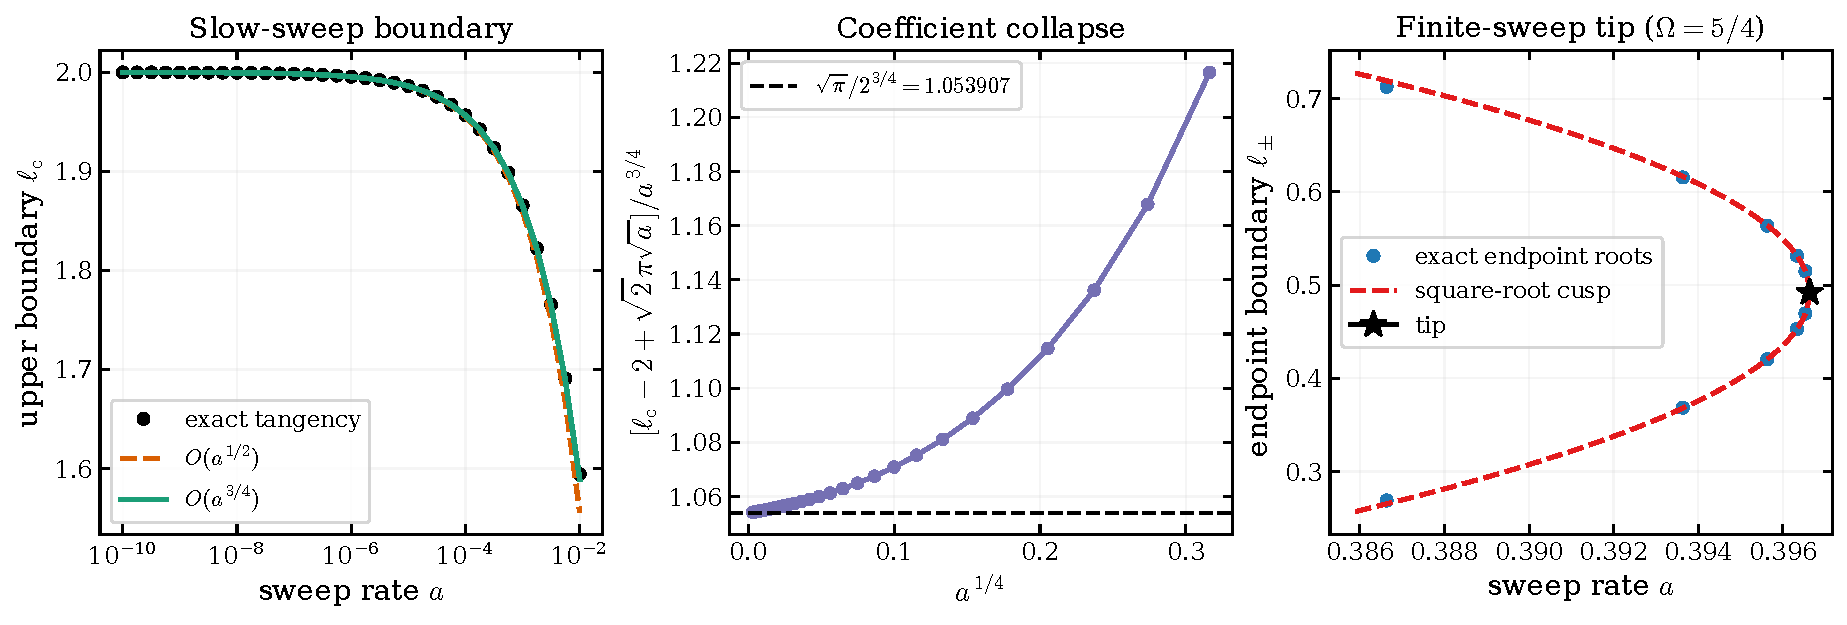
\includegraphics[width=\textwidth]{exact_boundary_asymptotics.pdf}
\caption{Controlled slow-sweep geometry. Left: numerically continued
double-tangency boundary and its
one- and two-term asymptotic approximations. Center: collapse onto the
analytical coefficient of \(a^{3/4}\). Right: square-root cusp at the
finite-sweep tip for \(\Omega_\Delta=5/4\).}
\label{fig:boundaryasymptotics}
\end{figure*}

\subsection{Uniform asymptotic control beyond the first lifted zero}
\label{subsec:uniformity}

At the \(n\)th zero \(s_n=n\pi/k\), the imaginary lift is
\begin{equation}
w_n=(-1)^{n+1}\frac{n^2\pi^2}{4k^4}.
\label{eq:wn}
\end{equation}
Thus, every fixed later zero is less favorable to a revival than the first.
This fixed-\(n\) statement alone is insufficient, because the number of
oscillation cells diverges as \(a\to0\). Appendix~\ref{app:uniform} closes
that gap with two overlapping estimates. For
\(N_\epsilon=\lfloor\epsilon^{-1/4}\rfloor\), Duhamel control gives
\begin{equation}
\sup_{\mathcal C_n}\Ree\{q\}
=-1+\frac1{n^2}+O(\epsilon^{1/2}),
\qquad 2\leq n\leq N_\epsilon.
\label{eq:earlyuniform}
\end{equation}
A weighted no-turning-point Liouville--Green basis then gives
\begin{equation}
\sup_{\mathcal C_n}\Ree\{q\}
\leq-1+C\epsilon^{1/2}\ln^{3/2}(1/\epsilon)
\label{eq:lateuniform}
\end{equation}
through the crossover
\(s=O[\epsilon^{-1/2}\sqrt{\ln(1/\epsilon)}]\). Here,
Liouville--Green means the controlled WKB representation of the scaled
equation \(U''+Q_\epsilon(s)U=0\) in the basis
\begin{equation}
\psi_\pm(s)=Q_\epsilon(s)^{-1/4}
\exp\!\left[\pm\ii\int_0^s\sqrt{Q_\epsilon(r)}\dd r\right].
\label{eq:LGbasis}
\end{equation}
This is the no-turning-point form of the standard Liouville--Green
construction~\cite{Olver1997}.
It is called ``no turning point'' because the complex coefficient
\(Q_\epsilon\) has no zero on the real crossover interval; hence a continuous
branch of \(\sqrt{Q_\epsilon}\) exists there. Unlike the local lifted-zero
expansion, this basis remains uniform across a number of oscillations that
diverges as \(a\to0\). Appendix~\ref{app:uniform} bounds its accumulated
variation and the associated remainder. At the crossover exit the solution
enters the attracting frozen Riccati branch with
\begin{equation}
|q-q_s|=O(\epsilon^2),
\qquad
q_s(\delta)=-\frac{\ell+\ii\delta}{2}
+\frac12\sqrt{(\ell+\ii\delta)^2-2\ell},
\label{eq:slowbranch}
\end{equation}
and \(\Ree\{q_s\}<0\) for every \(\delta>0\). An invariant Riccati tube preserves
this sign to the end of the sweep. Consequently, in the asymptotic regime and
at the critical value in
Eq.~\eqref{eq:mainboundary}, the first tangency has zero height while all later
maxima retain a strictly negative margin. This makes the matched expansion
uniform over the full finite linear sweep as \(a\to0^+\); it is distinct from
the finite-\(a\) numerical branch certification described in
Sec.~\ref{sec:finitesweep}.

The Supplemental Material tests the two leading fractional coefficients for analytic control profiles with the same local slope and records the corresponding exactly solvable examples.

\section{Finite-sweep geometry}
\label{sec:finitesweep}

The finite protocol has boundary mechanisms that are invisible in the
infinite-time constant-resonance problem. We resolve them here for
\(\Omega_\Delta=5/4\), the value used below for the representative trajectory. We
use ``boundary structure'' rather than topology: no topological invariant is
being defined. The issue is the geometric organization of distinct
zero-level mechanisms in the \((a,\ell)\) plane. The interior tangency reaches the stopping time when
\begin{equation}
\Ree\{q(\Omega_\Delta/a;\ell,a)\}=0,
\qquad
\partial_\tau\Ree\{q(\Omega_\Delta/a;\ell,a)\}=0.
\label{eq:mechanismswitch}
\end{equation}
Equations~\eqref{eq:mechanismswitch} define the mechanism-switch point
\((a_{\rm sw},\ell_{\rm sw})\) without a numerical phase-grid criterion; its
location for \(\Omega_\Delta=5/4\) is marked in Fig.~\ref{fig:finiteboundary}.

\begin{figure*}[t]
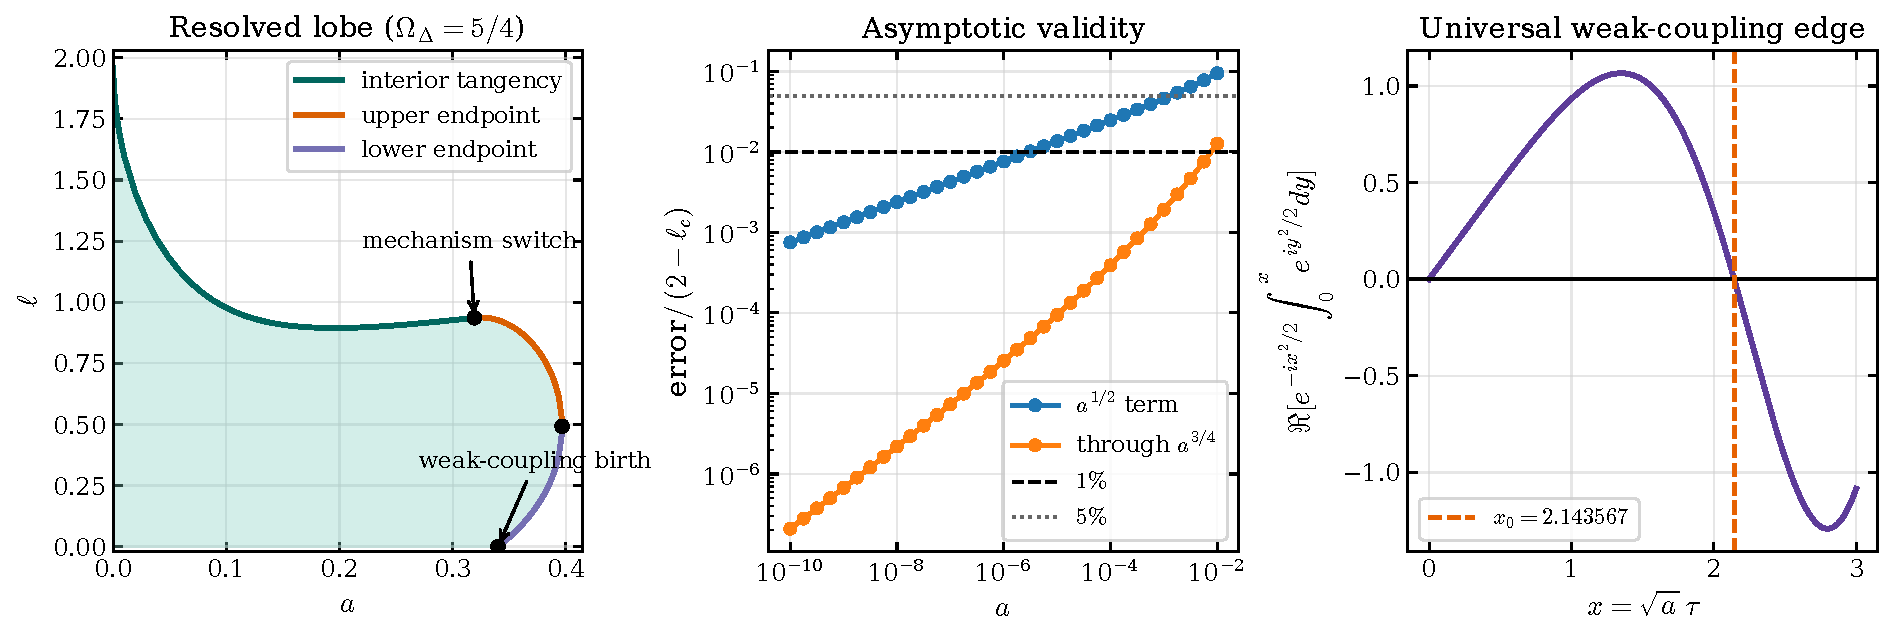
\includegraphics[width=\textwidth]{finite_sweep_boundary_structure.pdf}
\caption{Exactly defined and numerically resolved finite-sweep boundary for
\(\Omega_\Delta=5/4\). Left: non-Markovian lobe and switch from
interior-tangency to endpoint control at
\((\ell_{\rm sw},a_{\rm sw})=(0.936188,0.319102)\), endpoint-branch birth
at \(a_0=0.340052\), and cusp tip at
\((\ell_t,a_t)=(0.492257,0.396633)\).
Center: normalized errors of the one- and two-term slow-sweep laws. Right:
Fresnel function generating the weak-coupling endpoint birth.}
\label{fig:finiteboundary}
\end{figure*}

\begin{figure*}[t]
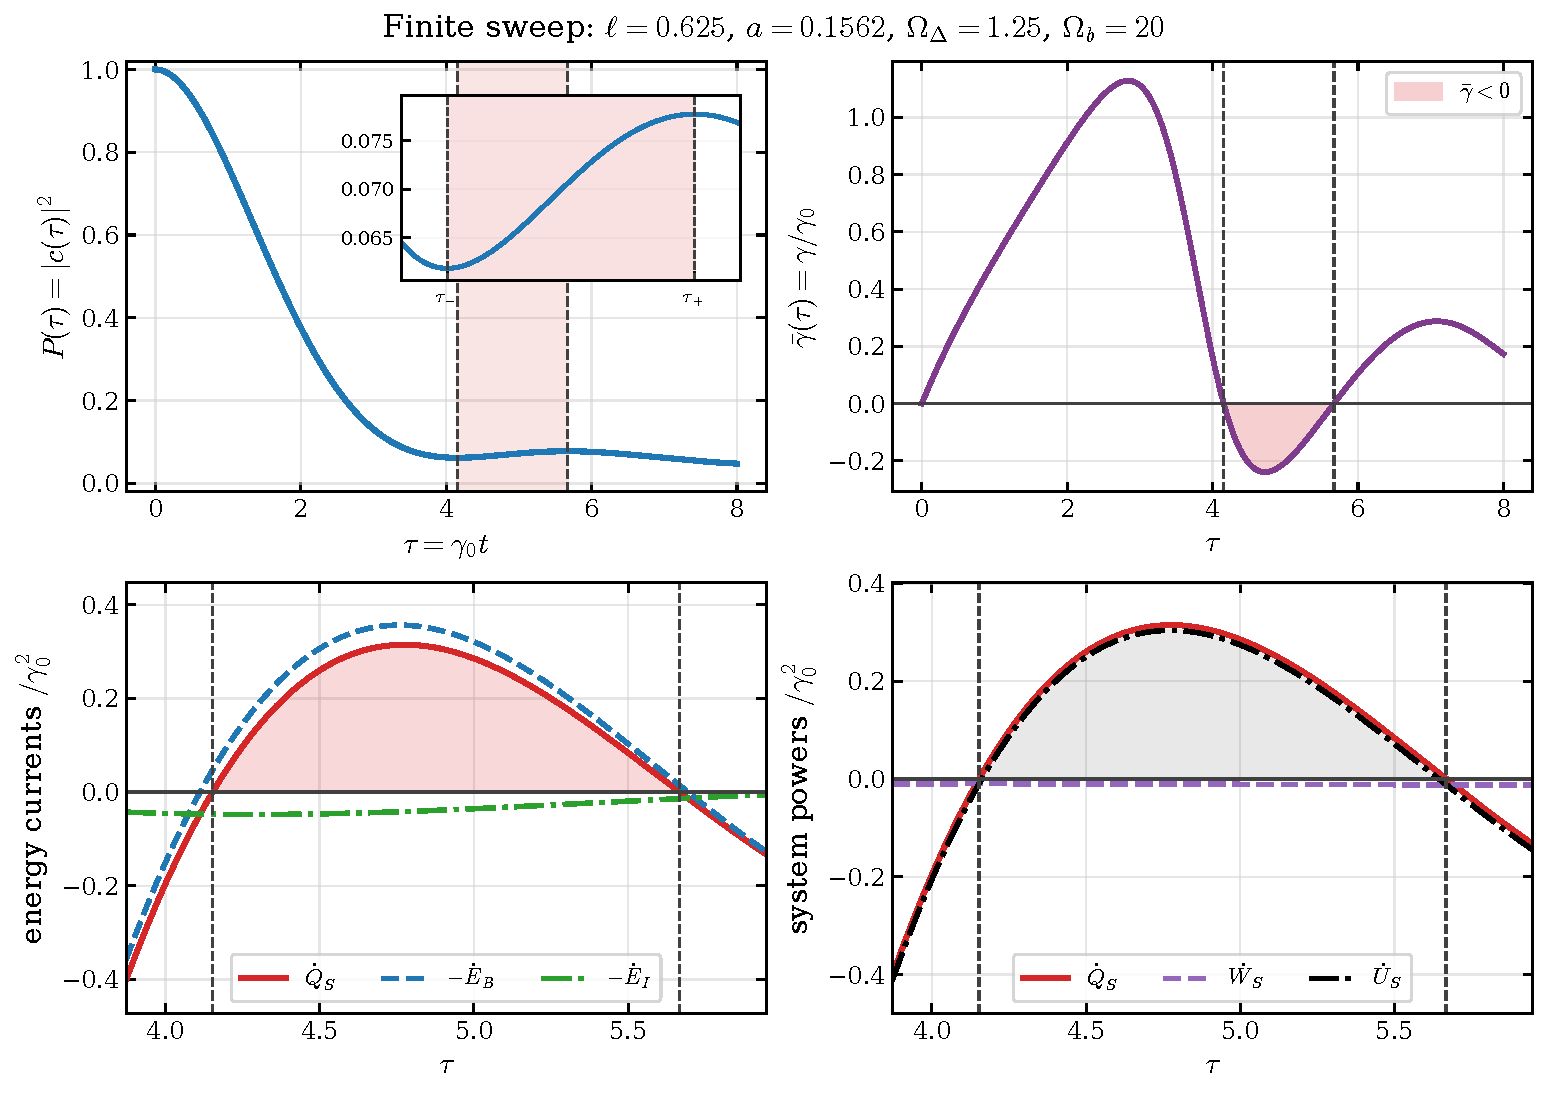
\includegraphics[width=0.98\textwidth]{thesis_exact_energy_correlation.pdf}
\caption{Representative positive-gap trajectory for
\((\ell,a,\Omega_\Delta,\Omega_b)=(5/8,5/32,5/4,20)\). The negative-rate
and revival interval is
\(4.15307<\tau<5.66767\), over which the population rises from
\(0.0618297\) to \(0.0777680\). The population inset resolves the revival.
The lower-left panel displays separately
the heat-like bare-system current \(\dot Q_S\), reservoir-to-system current
\(-\dot E_B\), and interaction-energy release \(-\dot E_I\), which obey
\(\dot Q_S=-\dot E_B-\dot E_I\). The lower-right panel instead displays
\(\dot U_S=\dot W_S+\dot Q_S\), showing that a positive heat-like current and
an increase of total qubit energy are distinct sign tests. Dashed vertical
lines mark \(\tau_-\) and \(\tau_+\).}
\label{fig:representativetrajectory}
\end{figure*}

Continuation of Eq.~\eqref{eq:exactODE} together with its variational
equations gives
\begin{equation}
(\ell_{\rm sw},a_{\rm sw})=(0.936188,0.319102).
\label{eq:switchcoordinates}
\end{equation}
We used DOP853 integration with relative and absolute tolerances
\(2\times10^{-10}\) and \(2\times10^{-12}\), respectively, and solved the
two residual equations to below \(10^{-10}\); halving both tolerances changes
the displayed coordinates by less than the last quoted digit.
For \(a>a_{\rm sw}\), the physical upper boundary is determined by the
endpoint rather than the continuation of an inaccessible later tangency. The weak-coupling edge follows analytically from
\(q=\ell r_1+O(\ell^2)\):
\begin{equation}
r_1(\tau)=-\frac12\ee^{-\ii a\tau^2/2}
\int_0^\tau\ee^{\ii au^2/2}\dd u.
\label{eq:weakcoupling}
\end{equation}
With \(x=\sqrt a\,\tau\), its sign is controlled by the parameter-free
Fresnel function
\begin{equation}
H(x)=\Ree\left[
\ee^{-\ii x^2/2}\int_0^x\ee^{\ii y^2/2}\dd y
\right].
\label{eq:Fresnelfunction}
\end{equation}
Let \(x_0=2.14357\ldots\) denote the first positive zero of \(H\). The
endpoint branch is born at \(\ell=0\) when
\begin{equation}
a_0(\Omega_\Delta)=\left(\frac{\Omega_\Delta}{x_0}\right)^2,
\qquad a_0(5/4)=0.340052.
\label{eq:lowerbirth}
\end{equation}

Finally, the two endpoint roots merge at a cusp. If
\(g(\ell,a)=\Ree q(\Omega_\Delta/a;\ell,a)\), the tip
\((a_t,\ell_t)\) is defined exactly by \(g=\partial_\ell g=0\).
Taylor expansion about this double root gives
\begin{align}
\ell_\pm(a)&=\ell_t\pm C_t\sqrt{a_t-a}+O(a_t-a),
\nonumber\\
C_t&=\left.
\sqrt{\frac{2\,\partial_a g}{\partial_\ell^2g}}
\right|_{(\ell_t,a_t)}.
\label{eq:endpointcusp}
\end{align}
For \(\Omega_\Delta=5/4\), the numerically continued double root is
\begin{equation}
(\ell_t,a_t)=(0.492257,0.396633),
\label{eq:tipcoordinates}
\end{equation}
with the same residual and tolerance checks as the switch point.
The three numerically resolved regimes are therefore: interior-tangency control for
\(a<a_{\rm sw}\); one endpoint upper edge for
\(a_{\rm sw}<a<a_0\); and two endpoint edges for \(a_0<a<a_t\).

Figure~\ref{fig:finiteboundary} displays this boundary structure and
quantifies the useful range of the asymptotic expansion. Normalization by the
natural deficit \(2-\ell_c\) shows that including the explicit
\(a^{3/4}\) term extends the accurate range by several orders of magnitude
relative to the leading square-root term alone.

The Supplemental Material continues the switch, endpoint birth, and cusp conditions over the tested range $1\leq\Omega_\Delta\leq2$ and reports the range at which their ordering changes.

As a representative point, take the exact dynamical ratios
\((\ell,a,\Omega_\Delta)=(5/8,5/32,5/4)\) and the independent physical
carrier \(\Omega_b=20\), for which the final gap is
\(\omega_f/\gamma_0=18.75\) and \(\omega_b/\lambda=32\). Figure
\ref{fig:representativetrajectory} shows the resulting revival, the microscopic
partition of \(\dot Q_S\), and the distinct signs allowed for \(\dot Q_S\) and
\(\dot U_S\). Integrated measures and the illustrative rate-matched spectral
comparison are reported in the Supplemental Material.

\section{Markovian failure, experimental outlook, and conclusions}
\label{sec:Markovian}

\subsection{Frozen-reservoir Markovian benchmark}

The instantaneous frozen-reservoir vacuum Born--Markov approximation replaces
the exact memory kernel at each time by the stationary weak-coupling response
at the current detuning. Equivalently, it replaces the exact Riccati solution
by its local stationary value,
\begin{equation}
q_{\rm M}(\tau)=-\frac{\ell}{2(\ell+\ii a\tau)},
\qquad
\bar\gamma_{\rm M}(\tau)=\frac{\ell^2}{\ell^2+a^2\tau^2}>0.
\label{eq:Markovrate}
\end{equation}
For the linear sweep this gives
\begin{equation}
P_{\rm M}(\tau)=
\exp\left[-\frac{\ell}{a}
\arctan\left(\frac{a\tau}{\ell}\right)\right].
\label{eq:Markovpopulation}
\end{equation}
It is monotone for every \((a,\ell)\). Consequently, the instantaneous
Markovian theory predicts no critical lobe, no exceptional-point threshold,
no lifted-zero mechanism, no endpoint cusp, no probability revival, and no
positive heat-like return.

The disagreement is not merely quantitative. During an exact interval with
\(\bar\gamma<0\), Eq.~\eqref{eq:energybackflow} gives
\(\dot Q_S>0\), whereas Eq.~\eqref{eq:Markovrate} enforces
\(\dot Q_S^{\rm M}<0\). At Born order the interaction energy
\(E_I=2Ps\) is also removed from the balance, so \(-\dot E_B\) is
incorrectly identified with the heat-like bare-system current whenever
\(\dot E_I\) is appreciable. The Markovian model is recovered only after the
reservoir memory encoded in the pseudomode has been adiabatically eliminated;
it cannot decide whether a later population revival occurs or identify the
microscopic source of the positive heat-like current.

Illustrative rate-matched power-law reservoirs, commuting phase damping, and their numerical convergence tests are reported in the Supplemental Material; they delimit the scope of the Lorentzian-reservoir result without entering the critical-boundary derivation.

\subsection{Experimental outlook}

A direct population-level test can be implemented with a tunable qubit coupled
to a lossy cavity mode, which realizes the Lorentzian pseudomode in
Eq.~\eqref{eq:pseudomode}. After calibrating \(\gamma_0\) and the cavity
linewidth \(\lambda\), one prepares a single qubit excitation with the mode
near vacuum, sets \(\omega(0)=\omega_b\), and applies a chirp with
\(\Delta_f<\omega_b\). Repeated measurements of the full population trace,
fitted directly to Eq.~\eqref{eq:pseudomode}, locate the revival without
numerically differentiating noisy data near a population minimum. Scans of
the chirp and linewidth would map the critical lobe, test the
\(a^{1/2}+a^{3/4}\) law, and resolve the endpoint cusp by varying the sweep
range.

The population measurement alone certifies the sign of \(\dot Q_S\). A
microscopic partition of that current additionally requires the cavity output
and the phase-sensitive qubit--cavity correlator entering \(E_I\). Concrete
circuit-QED scales, thermal and dephasing requirements, and the corresponding
measurement protocol are given in the Supplemental Material.

\subsection{Conclusions}
\label{sec:conclusion}

We have derived the critical revival geometry of a frequency-swept qubit
coupled to an effective full-line Lorentzian reservoir. The boundary is not a smooth
perturbation of the static threshold. A chirp lifts the first zero of the
resonant survival amplitude into the complex plane and produces the fractional
law \(a^{1/2}+a^{3/4}\). A uniform logarithmic-derivative estimate controls
all later cells in the slow-sweep limit. At finite duration, numerical
continuation of the exact implicit conditions resolves the switch from an
interior tangency to endpoint control, the weak-coupling Fresnel birth, and a
terminal square-root cusp.

The pseudomode representation unifies these facts. The static threshold
\(\ell=2\) is an exceptional point of the exact one-excitation amplitude
generator, not a claim about the full extended Liouvillian spectrum. The
frequency sweep is a controlled \(\mathcal{PT}\)-breaking perturbation. The
first two fractional coefficients are universal with respect to the tested
analytic changes of the control profile that preserve its local slope; no
universality over arbitrary spectral densities is claimed. The Supplemental
Material documents those profile tests, finite-range reordering, an exact
multipseudomode extension for sums of displaced Lorentzians, and illustrative
rate-matched power-law trajectories. These extensions preserve the exact
channel identities but show that revival magnitudes and final populations are
spectrally dependent.

Energetically, \(\bar\gamma<0\) is exactly equivalent to
\(\dot Q_S>0\) for every initial state with nonzero excited population and
positive transition frequency. It is not equivalent to \(\dot U_S>0\),
because the chirp also performs work, and it does not imply that the reservoir
loses energy. Equation~\eqref{eq:energycounterexample} gives an explicit
counterexample: released interaction energy sustains \(\dot Q_S>0\) while the
bath gains energy and the downward sweep makes \(\dot U_S<0\). Useful work
cannot be identified with any one of these currents; switching, extraction,
and reset costs must be included in a complete cycle. The exact solution
therefore supplies a rigorous diagnostic for memory-assisted thermodynamic
protocols, not by itself a claim of net-work advantage.

An instantaneous Markovian master equation predicts a positive rate at every
time and consequently misses the entire lobe, its exceptional-point origin,
all fractional and cusp geometry, and the sign reversal of the heat-like
current. The model provides a direct example in which the standard
approximation is not merely inaccurate but qualitatively opposite to the exact
sweep-resolved dynamics.

\section*{Acknowledgments}

A.N.\ acknowledges support from Fondecyt Regular No.~1251131, Fondecyt
Exploraci\'on No.~13250014, and Anillo Tem\'atico ATE 250066.

\section*{Data availability}

The data, source files, software, and regression tests supporting this study
are provided in the reproducibility archive cited in
Ref.~\cite{DataArchive}. The archive contains the inputs needed to regenerate
all figures and Table~SII and to verify the analytical coordinates and energy
balances.

\appendix

\section{Parabolic-cylinder representation}
\label{app:weber}

Let
\begin{equation}
z_0=-\ee^{-\ii\pi/4}\frac{\ii\ell}{\sqrt a},
\qquad \eta=\ee^{-\ii\pi/4}\sqrt a.
\end{equation}
The coefficients in Eq.~\eqref{eq:Webersolution} are the unique solution of
\begin{equation}
\begin{pmatrix}
D_\nu(z_0)&D_\nu(-z_0)\\
\eta D_\nu'(z_0)&-\eta D_\nu'(-z_0)
\end{pmatrix}
\begin{pmatrix}A\\B\end{pmatrix}
=\begin{pmatrix}1\\\ell/2\end{pmatrix}.
\label{eq:ABsystem}
\end{equation}
Using \(D_\nu'(z)=zD_\nu(z)/2-D_{\nu+1}(z)\), the logarithmic derivative can
be evaluated without numerical differentiation:
\begin{equation}
q=-\frac\ell2-\frac{\ii a\tau}{2}
+\eta\frac{A D_\nu'(z)-B D_\nu'(-z)}
{A D_\nu(z)+B D_\nu(-z)}.
\label{eq:qWeber}
\end{equation}
For very small \(a\), the large imaginary order
\(\nu=\ii\ell/(2a)\) makes direct special-function evaluation ill-conditioned.
We therefore used Eq.~\eqref{eq:exactODE}, its exponentially desingularized
form, and Eq.~\eqref{eq:Riccati} as independent numerical representations.
At \(a=10^{-2}\), their values of \(q\) at the critical tangency agree within
\(3.2\times10^{-12}\).

\section{Second fractional coefficient}
\label{app:asymptotics}

Write \(\mu=\mu_0+\epsilon\mu_1+\epsilon^2\mu_2+\cdots\) and
\(\mathcal L=\dd^2/\dd s^2+k^2\), with
\(k^2=\mu_0/2\). The first correction to Eq.~\eqref{eq:Uzero} is
\begin{align}
\mathcal L U_1&=\left(\ii s-\frac{\mu_1}{2}\right)U_0,
\label{eq:U1equation}\\
U_1&=\cos(ks)+\ii w(s)-\frac{\mu_1}{2}z(s),\nonumber\\
z(s)&=-\frac{s\cos(ks)}{2k^2}
+\frac{\sin(ks)}{2k^3}.
\label{eq:zfunction}
\end{align}
The cosine in \(U_1\) enforces \(U_1(0)=1\), inherited from
\(U(0)=\epsilon\). The two particular solutions are explicitly
\begin{align}
w(s)&=\int_0^sG(s,r)\,rU_0(r)\dd r,
\nonumber\\
z(s)&=\int_0^sG(s,r)\,U_0(r)\dd r,
\label{eq:wzGreen}
\end{align}
where \(G\) is Eq.~\eqref{eq:criticalGreenfunction}. Thus the phrase
``Green-function integral'' refers simply to the exact inverse of the
constant-coefficient operator \(\mathcal L\), not to an additional
approximation.
At \(s_0=\pi/k\),
\begin{equation}
d:=w'(s_0)=\frac{\pi}{4k^3},
\qquad z(s_0)=\frac{\pi}{2k^3},
\qquad z'(s_0)=0.
\label{eq:criticalvalues}
\end{equation}
If \(v_2=\Imm U_2\), the only Green-function value needed at the next order is
\begin{equation}
v_2(s_0)=\mu_1A_1,
\qquad
A_1=-\frac{3\pi^2}{16k^6}.
\label{eq:A1}
\end{equation}
Indeed, Eq.~\eqref{eq:U2hierarchy} gives
\begin{align}
U_2(s)&=U_2^{\rm hom}(s)
+\int_0^sG(s,r)\mathcal S_2(r)\dd r,
\nonumber\\
\mathcal S_2(r)&=\left(\ii r-\frac{\mu_1}{2}\right)U_1(r)
\nonumber\\
&\quad+\left(\frac{\mu_0^2}{4}+\frac{\ii}{2}
-\frac{\mu_2}{2}\right)U_0(r),
\label{eq:U2Green}
\end{align}
and taking its imaginary part at \(s_0\) reduces the elementary sine
integrals to Eq.~\eqref{eq:A1}. The homogeneous term enforces the order-two
initial derivative and vanishes at \(s_0\).
After absorbing the real displacement into the inner coordinate, the maximal
logarithmic population rate becomes
\begin{equation}
\max_\xi\Ree q=
2\epsilon\left[d+\mu_1(d^2-A_1)\right]+O(\epsilon^2).
\label{eq:qnext}
\end{equation}
The tangency condition therefore gives
\begin{equation}
\mu_1=\frac{d}{A_1-d^2}
=-\frac{k^3}{\pi}
=-\frac{\sqrt\pi}{2^{3/4}},
\end{equation}
which proves the second term in Eq.~\eqref{eq:mainboundary}.

\section{Uniform crossover and late-time sign control}
\label{app:uniform}

We state the estimate for a smooth saturating extension of the finite linear
sweep. Since the extension begins after \(\tau_f\), it does not modify the
physical dynamics. More generally, let
\(\delta_a(\tau)=d f(a\tau/d)\), where
\(f\in C^3([0,\infty))\), \(f(0)=0\), \(f'(0)=1\), \(f'\geq0\), the first
three derivatives are bounded, and \(f\) approaches a positive constant.
Assume \((2-\ell)/\epsilon^2\to\mu_0\), where
\(\epsilon=a^{1/4}\).

Fix \(L>L_0\), with \(L_0\) independent of \(\epsilon\), and set
\begin{align}
S_\epsilon&=L\epsilon^{-1/2}\sqrt{\ln(1/\epsilon)},
\qquad N_\epsilon=\lfloor\epsilon^{-1/4}\rfloor,
\nonumber\\
k_\epsilon^2&=\frac{2-\ell}{2\epsilon^2}.
\label{eq:splitindices}
\end{align}
Then \(k_\epsilon\to k_0\), where
\(k_0^2=\mu_0/2=\pi/\sqrt2\). The constant \(L_0\) is chosen once so that
the Liouville--Green damping accumulated by \(S_\epsilon\) dominates the
algebraic matching errors below; it does not grow as \(\epsilon\to0\).
There are \(C,\epsilon_0>0\), independent of the oscillation-cell index, such
that for \(0<\epsilon<\epsilon_0\),
\begin{align}
\sup_{\mathcal C_n}\Ree q
&=-1+\frac1{n^2}+O(\epsilon^{1/2}),
&&2\leq n\leq N_\epsilon,
\label{eq:appendixearly}\\
\sup_{\mathcal C_n}\Ree q
&\leq-1+C\epsilon^{1/2}\ln^{3/2}(1/\epsilon),
&&N_\epsilon\leq n\leq k_0S_\epsilon/\pi.
\label{eq:appendixlate}
\end{align}
In particular, the entire set of later cells has limiting upper bound
\(-3/4\).

For completeness, the main ingredients are as follows. On the crossover
interval the scaled equation has coefficient
\begin{align}
Q_\epsilon(s)&=k_\epsilon^2-\frac{\ii\ell\epsilon s}{2}
+R_\epsilon(s),\nonumber\\
|R_\epsilon|+(1+s)^{-1}|R_\epsilon'|
&\leq C\epsilon^2(1+s^2).
\label{eq:Qremainder}
\end{align}
For \(n\leq N_\epsilon\), Duhamel's formula about
\(U_0=\sin(k_\epsilon s)/k_\epsilon\) resolves each lifted zero. The lift has
size \(\epsilon n^2\), while the remainder after division by the local
solution contributes only \(O(\epsilon n^2)\), proving
Eq.~\eqref{eq:appendixearly}.

For \(n\geq N_\epsilon\), set \(p_a=\sqrt{Q_\epsilon}\), using the branch
continued from \(p_a(0)>0\). The imaginary chirp term keeps
\(Q_\epsilon(s)\) away from zero for real \(s>0\) in the crossover, so no
turning-point connection formula is required. Substitution of
\(p_a^{-1/2}\exp(\pm\ii\int p_a\dd s)\) into the scaled equation leaves the
standard Liouville--Green residual
\begin{equation}
\mathcal R_a=
\frac{3(p_a')^2}{4p_a^3}-\frac{p_a''}{2p_a^2}.
\label{eq:LGresidual}
\end{equation}
Variation of constants around this basis is controlled by its integral,
\begin{equation}
\int_0^{S_\epsilon}
|\mathcal R_a(s)|\dd s
=O\!\left(\epsilon^{3/2}\sqrt{\ln(1/\epsilon)}\right).
\label{eq:variationintegral}
\end{equation}
Define the accumulated imaginary Liouville--Green phase by
\begin{equation}
\Theta_a(s)=\left|\Im\int_0^s p_a(r)\dd r\right|.
\label{eq:LGphase}
\end{equation}
At the late-cell entry, \(\Theta_a(s_n)\geq c\epsilon^{1/2}\), so the weighted
basis bounds can be divided
by the exact solution without a small-denominator loss. This proves
Eq.~\eqref{eq:appendixlate}. At the exit,
\begin{equation}
\tau_m=\frac{S_\epsilon}{\epsilon},\qquad
r_m:=\left|q(\tau_m)-q_s[\delta_a(\tau_m)]\right|
\leq C\epsilon^2.
\label{eq:entrybound}
\end{equation}

To control the remaining tail, write \(e=q-q_s(\delta)\) and
\(\Delta=\sqrt{(\ell+\ii\delta)^2-2\ell}=u+\ii v\), \(u>0\). The exact
Riccati equation gives
\begin{equation}
e'=-\Delta e-e^2-q_{s,\delta}\delta'.
\end{equation}
For \(r=|e|\), its upper Dini derivative satisfies
\begin{equation}
D^+r\leq-u r+r^2+|q_{s,\delta}\delta'|.
\label{eq:tubeinequality}
\end{equation}
Let \(u_*\) and \(m_*\) be the minimum of \(u\) and
\(-\Ree q_s\) on the tail, and let
\(F_*\) be the maximum forcing. If \(u_*^2>4F_*\), define
\begin{equation}
R_\pm=\frac{u_*\pm\sqrt{u_*^2-4F_*}}2.
\end{equation}
The comparison principle gives the invariant-tube criterion
\begin{equation}
\max\{r_m,R_-\}<\min\{m_*,R_+\}
\quad\Longrightarrow\quad
\Ree q(\tau)<0
\label{eq:tubecriterion}
\end{equation}
for every later time. Equation~\eqref{eq:entrybound} satisfies this criterion
for all sufficiently small \(a\), completing the global sign proof.



\begin{thebibliography}{99}

\bibitem{Breuer2009}
H.-P. Breuer, E.-M. Laine, and J. Piilo,
Measure for the degree of non-Markovian behavior of quantum processes in open
systems,
Phys. Rev. Lett. \textbf{103}, 210401 (2009).

\bibitem{Rivas2010}
\'A. Rivas, S. F. Huelga, and M. B. Plenio,
Entanglement and non-Markovianity of quantum evolutions,
Phys. Rev. Lett. \textbf{105}, 050403 (2010).

\bibitem{Bylicka2014}
B. Bylicka, D. Chru\'sci\'nski, and S. Maniscalco,
Non-Markovianity and reservoir memory of quantum channels,
Sci. Rep. \textbf{4}, 5720 (2014).

\bibitem{Strasberg2019}
P. Strasberg and M. Esposito,
Non-Markovianity and negative entropy production rates,
Phys. Rev. E \textbf{99}, 012120 (2019).

\bibitem{Ptaszynski2022}
K. Ptaszy\'nski,
Non-Markovian thermal operations boosting the performance of quantum heat
engines,
Phys. Rev. E \textbf{106}, 014114 (2022).

\bibitem{Picatoste2024}
I. A. Picatoste, A. Colla, and H.-P. Breuer,
Dynamically emergent quantum thermodynamics: Non-Markovian Otto cycle,
Phys. Rev. Research \textbf{6}, 013258 (2024).

\bibitem{ZambonAdesso2025}
G. Zambon and G. Adesso,
Quantum processes as thermodynamic resources: The role of non-Markovianity,
Phys. Rev. Lett. \textbf{134}, 200401 (2025).

\bibitem{Guarnieri2016}
G. Guarnieri, C. Uchiyama, and B. Vacchini,
Energy backflow and non-Markovian dynamics,
Phys. Rev. A \textbf{93}, 012118 (2016).

\bibitem{Schmidt2016}
R. Schmidt, S. Maniscalco, and T. Ala-Nissil\"a,
Heat flux and information backflow in cold environments,
Phys. Rev. A \textbf{94}, 010101(R) (2016).

\bibitem{Mortezapour2018}
A. Mortezapour and R. Lo Franco,
Protecting quantum resources via frequency modulation of qubits in leaky
cavities,
Sci. Rep. \textbf{8}, 14304 (2018).

\bibitem{Zhang2026}
X. Q. Zhang and W. W. Cheng,
Enhancing precision of environment parameters estimation via frequency
modulation,
Ann. Phys. \textbf{488}, 170396 (2026).

\newpage
\bibitem{Khazaei2026}
M. Khazaei Shadfar \textit{et al.},
Preserving quantum coherence in thermal noisy systems via qubit frequency
modulation,
Adv. Quantum Technol. \textbf{9}, e70349 (2026).

\bibitem{Haikka2011}
P. Haikka, J. D. Cresser, and S. Maniscalco,
Comparing different non-Markovianity measures in a driven qubit system,
Phys. Rev. A \textbf{83}, 012112 (2011).

\bibitem{Li2010}
J.-G. Li, J. Zou, and B. Shao,
Non-Markovianity of the damped Jaynes--Cummings model with detuning,
Phys. Rev. A \textbf{81}, 062124 (2010).

\bibitem{Amati2024}
G. Amati,
Dynamical signatures of non-Markovianity in a dissipative-driven qubit,
Phys. Rev. A \textbf{109}, 052433 (2024).

\bibitem{Garraway1997}
B. M. Garraway,
Nonperturbative decay of an atomic system in a cavity,
Phys. Rev. A \textbf{55}, 2290 (1997).

\bibitem{Pleasance2020}
G. Pleasance, B. M. Garraway, and F. Petruccione,
Generalized theory of pseudomodes for exact descriptions of non-Markovian
quantum processes,
Phys. Rev. Research \textbf{2}, 043058 (2020).

\bibitem{TalknerHanggi2020}
P. Talkner and P. H\"anggi,
Colloquium: Statistical mechanics and thermodynamics at strong coupling:
Quantum and classical,
Rev. Mod. Phys. \textbf{92}, 041002 (2020).

\bibitem{Campbell2018}
S. Campbell, F. Ciccarello, G. M. Palma, and B. Vacchini,
System--environment correlations and Markovian embedding of quantum
non-Markovian dynamics,
Phys. Rev. A \textbf{98}, 012142 (2018).

\bibitem{SupplementalMaterial}
See Supplemental Material for control-profile robustness, finite-range and
spectral-scope checks, integrated currents, numerical certification, and
microscopic bath reconstruction.

\bibitem{NIST2010}
F. W. J. Olver, D. W. Lozier, R. F. Boisvert, and C. W. Clark, eds.,
\textit{NIST Handbook of Mathematical Functions}
(Cambridge University Press, Cambridge, 2010).

\bibitem{BreuerPetruccione2002}
H.-P. Breuer and F. Petruccione,
\textit{The Theory of Open Quantum Systems}
(Oxford University Press, Oxford, 2002).

\bibitem{Lin2025}
J.-D. Lin, P.-C. Kuo, N. Lambert, A. Miranowicz, F. Nori, and Y.-N. Chen,
Non-Markovian quantum exceptional points,
Nat. Commun. \textbf{16}, 1289 (2025).

\bibitem{ZhangEP2025}
H.-L. Zhang, P.-R. Han, F. Wu, W. Ning, Z.-B. Yang, and S.-B. Zheng,
Experimental observation of non-Markovian quantum exceptional points,
Phys. Rev. Lett. \textbf{135}, 230203 (2025).

\bibitem{Heiss2012}
W. D. Heiss,
The physics of exceptional points,
J. Phys. A: Math. Theor. \textbf{45}, 444016 (2012).

\bibitem{Minganti2022}
F. Minganti, D. Huybrechts, C. Elouard, F. Nori, and I. I. Arkhipov,
Creating and controlling exceptional points of non-Hermitian Hamiltonians via
homodyne Lindbladian invariance,
Phys. Rev. A \textbf{106}, 042210 (2022).

\bibitem{Olver1997}
F. W. J. Olver,
\textit{Asymptotics and Special Functions}
(A K Peters, Wellesley, MA, 1997).

\bibitem{Esposito2010}
M. Esposito, K. Lindenberg, and C. Van den Broeck,
Entropy production as correlation between system and reservoir,
New J. Phys. \textbf{12}, 013013 (2010).

\bibitem{Ptaszynski2019}
K. Ptaszy\'nski and M. Esposito,
Entropy production in open systems: The predominant role of
intra-environment correlations,
Phys. Rev. Lett. \textbf{123}, 200603 (2019).

\bibitem{DataArchive}
F. Ahumada, F. Barra, and A. Norambuena,
Reproducibility archive for this work,
DOI: \texttt{DOI\_TO\_BE\_INSERTED\_AFTER\_DEPOSIT}.

\end{thebibliography}

\end{document}
